\chapter{Apéndice B: Pruebas Funcionales Realizadas}
\label{apendiceB}
\lhead{Apéndice B. \emph{Pruebas Funcionales Realizadas}}

\subsection{Pruebas funcionales}

En esta sección se explicarán las pruebas funcionales aplicadas a cada
una de la funciones construidas en el sistema.

\subsubsection{Filtro HTTP/GET}

Para probar el filtro de tipo HTTP/GET se tomó la base de datos,
\textbf{db1.pcap}, que contiene tanto paquetes HTTP/GET, como paquetes correspondientes a la sesión HTTP. La prueba consistió en pasarle a la función construida la base de datos de paquetes para que esta imprimiera los URIs de las peticiones HTTP/GET que estuviesen contenidas en la misma. En la
figura \ref{fig:filtroHTTP} se muestra un esquema de la prueba que se realizó.

\begin{figure}[!htb]
\begin{center}
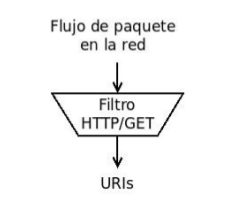
\includegraphics[width=2in]{./img/filtroHTTP.png}
\caption{Esquema de pruebas realizadas al filtro HTTP/GET.}
\label{fig:filtroHTTP}
\end{center}
\end{figure}

\subsubsection{Lectura de archivos}

La lectura de los archivos es de suma importancia, ya que el sistema utiliza un modelo de normalidad y un conjunto de parámetros que se introducen
al mismo a tráves de archivos.
La manera en la que se probó esta función consistió en leer ambos archivos de textos necesarios por el sistema: ``config'' y ``modeloBro.log'' y luego se imprimieron las tablas resultantes de la lectura de los mismos.
En la figura \ref{fig:configFile}, se puede observar el archivo ``config'' que leerá la función de lectura del sistema y en la figura \ref{fig:configResult}, se puede apreciar la forma en la
que la misma almacenó los datos en la tabla correspondiente.
Por otra parte, en la figura \ref{fig:modelFile}, está el archivo ``modeloBro.log'' que fué utilizado en la prueba realizada, mientras que en la figura \ref{fig:modelResult} se muestra el resultado arrojado por la misma.

\begin{figure}[!htb]
\begin{center}
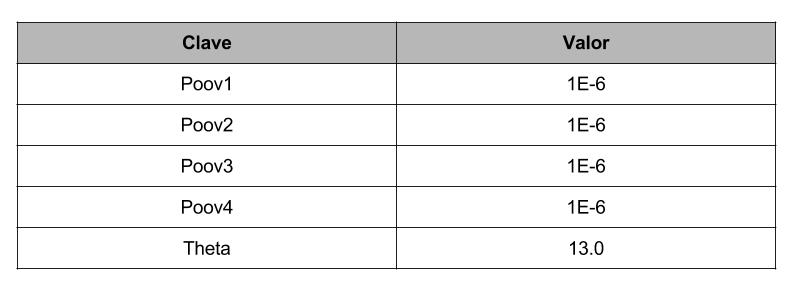
\includegraphics[width=3in]{./img/configFile.jpg}
\caption{Archivo ``config''.}
\label{fig:configFile}
\end{center}
\end{figure}

\begin{figure}[!htb]
\begin{center}
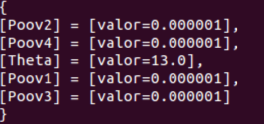
\includegraphics[width=3in]{./img/tablaConfig.png}
\caption{Tabla que contiene información del archivo ``config''.}
\label{fig:configResult}
\end{center}
\end{figure}

\begin{figure}[!htb]
\begin{center}
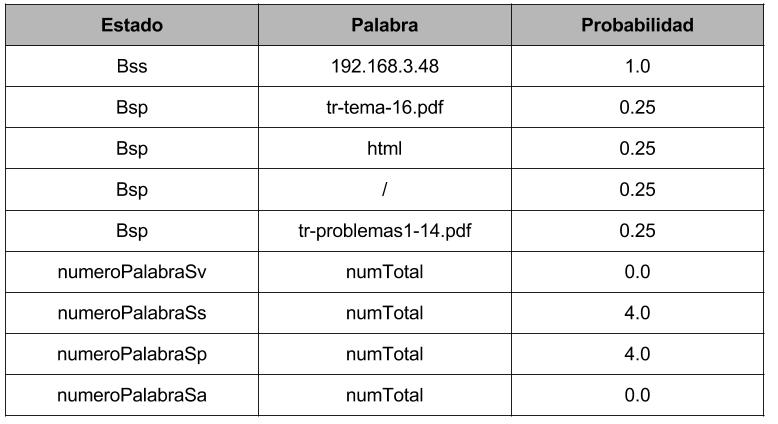
\includegraphics[width=3in]{./img/modeloOffline.jpg}
\caption{Archivo ``modeloBro.log''.}
\label{fig:modelFile}
\end{center}
\end{figure}

\begin{figure}[!htb]
\begin{center}
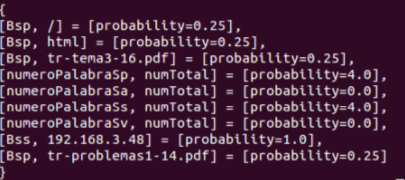
\includegraphics[width=3in]{./img/tablaModeloBro.png}
\caption{Tabla que contiene información del archivo ``modeloBro.log''.}
\label{fig:modelResult}
\end{center}
\end{figure}

\subsubsection{Módulo de segmentación}

Como se mencionó en los secciones anteriores, el modulo de segmentación
cuenta con dos funciones principales: la función de normalización y la de
segmentación. A continuación se mostrará la manera en la que se probó cada una de las funciones.

\subsubsection*{Función de normalización}

Las pruebas realizadas a la función de normalización consistió en realizar una lista de URIs sin normalizar, ingresarlos como parámetros a la función y observar los resultados arrojados por la misma.
La lista de URIs utilizados en esta prueba se pueden observar en la figura \ref{fig:uriSinNorm}. Por otra parte, los resultados arrojados por la misma se muestran en la
figura \ref{fig:uriNorm}.

\begin{figure}[!htb]
\begin{center}
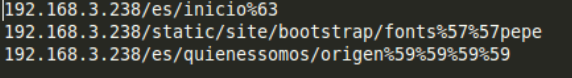
\includegraphics[width=3in]{./img/uriSinNorm.png}
\caption{URIs sin normalizar.}
\label{fig:uriSinNorm}
\end{center}
\end{figure}

\begin{figure}[!htb]
\begin{center}
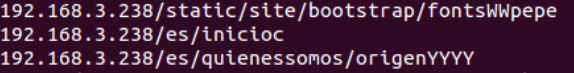
\includegraphics[width=3in]{./img/uriNorm.png}
\caption{URIs normalizados.}
\label{fig:uriNorm}
\end{center}
\end{figure}


\subsubsection*{Función de segmentación}

La pruebas realizadas a la función de segmentación, consistieron en ingresarle un conjunto de URIs a la misma y observar la manera en la que
esta los segmentaba.

\subsubsection{Módulo de entrenamiento}
\subsubsection*{Modo ``Offline''}
Como se pudo observar en los secciones anteriores, el módulo de entrenamiento esta conformado por una función, ``entrenarOffline'', que que se
encarga de hacer la llamada a función de: ``entrenamientoOffline'', ``evaluarProbabilidad'', ``escribirArchivoOffline''.
Para probar la función, ``entrenamientoOffline'', se construyeron una serie de datos de tipo ``UriSegmentado'' (fig. \ref{fig:uriSegmentado}), provenientes de la base de datos \textbf{db3.pcap} y le fueron pasados como parámetro de entrada a la misma. Una vez procesados los datos, se observó la salida de la misma para verificar la correctitud.

Por otra parte, para probar la función ``evaluarProbabilidad'', se tomaron los resultados arrojados por ``entrenamientoOffline'' y se
observó el resultado que arrojaba la misma. 

La prueba que se le realizó a ``escribirArchivoOffline'', consistió en tomar el resultado arrojado por ``evaluarProbabilidad'' y observar el
archivo de salida que escribía dicha función. 

\subsubsection*{Modo ``Online''}
Al igual que el modo ``Offline'', el modo ``Online'' esta conformado por
una función,``entrenarOnline'', que se encarga de hacer la llamada a función
del resto:``entrenamientoOnline'',``escribirArchivoOnline''
Las pruebas de ``entrenamientoOnline'' consistieron en darle un modelo de normalidad y un conjunto de estructura
de tipo ``UriSegmentado'' y observar la salida que arrojaba la misma.

Para probar la función ``escribirArchivoOnline'', se tomó el resultado arrojado por ``entrenamientoOnline'' y se observó el archivo de salida escrito por la misma.
\subsubsection{Módulo de evaluación}

El modulo de evaluación consta de una función general, llamada ``evaluacion'' que se encarga de hacer la llamada a función de: ``epsiloSumatoria'',
``calcularIndiceAnormalidad'', ``evaluarIndiceAnormalidad'' y ``escribirReporte'', que a su vez se encargan de realizar el trabajo del módulo de evaluación.
Para probar la función ``epsiloSumatoria'', se ingresó un conjunto de datos de tipo de tipo ``UriSegmentado'', un modelo de normalidad previamente leído, un valor para el epsilon, y un conjunto de estado del autómata para observar los resultados que arrojaba la misma.
Para la prueba de la función ``calcularIndiceAnormalidad'', se tomaron
los resultados proporcionados por la función ``epsiloSumatoria'' y se observará el resultado obtenido.

Tanto los resultados obtenidos por ``epsiloSumatoria'' por ``calcularIndiceAnormalidad'' fueron verificados calculando de manera manual los valores
que estas funciones calculan, haciendo uso de las expresiones correspondientes.
Las pruebas de la función ``evaluarIndiceAnormalidad'' consistieron en
darle un  índice de anormalidad y un valor del parámetro $\theta$, como los que
se muestran en la figura \ref{fig:archivoConfig} y verificar si la misma clasificaba de manera adecuada.
Finalmente, para realizar la prueba de ``escribirReporte'' se le pasó una serie de URIs pertenecientes a la base de datos \textbf{db1.pcap}. Una vez realizado
esto, se observó el archivo de salida escrito por dicha función.
